\chapter{Deep Multi-Agent RL Experiments}

All of the methods discussed in this work are typically implemented in function approximation
settings.
Hence, it is important to evaluate if the observed performance improvements carry over when the
policy parameters, and the value approximation are both represented using neural networks.

Expanding on our the observations from the tabular experiments, we proceed to evaluate the
algorithms in large-scale 2p0s games to answer question~\ref{qn3}.
For the neural experiments, we study the effect of the NeuRD-fix, and the utilization of
Optimistic-variants of popular optimizers (Optimistic-SGD, and Optimistic-Adam) when paired with
deep RL algorithms.

\section{Experimental Domains}
In the tabular experiments, we evaluated the algorithms as reinforcement learning methods in
normal-form games.
In this section, we evaluate the deep RL variant of these algorithms in extensive-form games.
EFGs have been used as common benchmark and milestones in designing and evaluating multi-agent
reinforcement learning.
\fillin{Should I expand on this?}
% A major achievement in recent times for reinforcement learning methods in large-scale game benchmarks was 
% AlphaGo's performance against professional Go players including winning against the world champion. 
We follow the suit of~\cite{sokotaUnified2023}, and choose four 2p0s EFGs for the evaluation,
namely - Kuhn Poker, Abrupt Dark Hex, and Phantom Tic-tac-toe.
Kuhn Poker, and 2x2 Dark Hex are smaller benchmarks that were used to test, and tune the
algorithms.
Phantom Tic-tac-toe, and 3x3 Dark Hex, are large-scale benchmarks that are used here to evaluate
the scalability, and stability of these algorithms in converging to an equilibrium.
Please refer to Appendix~\ref{apx:gamedesc} for an overview of these games.

\section{Evaluation Metrics}
The measures used in tabular experiments are harder to compute for large-scale EFGs.
Distance to an equilibrium point is harder to compute due to the absence of a unique equilibrium
point.
For larger games, the computation of exact best responses to measure the exact exploitability is
prohibitive due to the large state space.
However, we can approximate the exploitability computation if we can approximate the best response
for a given fixed policy.

\subsection{Approximate Exploitability}
For poker games, a local best response approximator (LBR)~\cite{lisyEquilibrium2017} has been
commonly used in place of an exact best response computation by combining local search along with
truncation based on a heuristic value function.
However, the value function is based on poker domain-specific knowledge, and does not translate to
other games.
Instead, an alternative LBR formulation was proposed in~\cite{timbersApproximate2022} that uses
MCTS~\footnote{It uses an extension of MCTS to imperfect-information settings called information
	state MCTS (ISMCTS)~\cite{cowlingInformation2012}} and an approximate learnt value function.
The exploitability is then computed by

Then the exploitability can be
approximated by sampling trajectories and measuring the average reward the best response agent
acheived against the exploited policy.
In our experiments, we train the best response agent against the fixed joint-policy learn through
self-play.
Let $\pi_{BR}$ be a learnt best-response approximator, and $\pi_{fixed}=(\pi_1, \pi_2)$ be the
joint policy to be exploited, then the approximate exploitability is given by:
\begin{equation}
	\label{eqn:appxexp} \text{Exp}_{appx} (\pi_{BR}, \pi_{fixed}) = \frac{1}{N} \left[ \sum_{i=1}^{N/2}
		\E_{a \sim \pi_1, \pi_{BR}} [R] + \sum_{i=1}^{N/2} \E_{a \sim \pi_{BR}, \pi_2} [R] \right]
\end{equation} \fillin{TBD: rephrase the equation in terms of cumulative episodic rewards.
}

\section{Experiment Setup}
Due to the strong performance exhibited by MMD~\cite{sokotaUnified2023} as a deep MARL algorithm
for 2p0s games, we consider vanilla-MMD to be our baseline.
For a proper comparison of MMD's performance against the proposed algorithms, we setup our
experiments following~\cite{sokotaUnified2023}, and we outline the various implementation details,
and experimental choices made in the former work here.

MMD was implemented as a modification of RLLib's~\cite{liangRLlib2018} PPO, by modifying the
entropy, and KL annealing schedules.
RLLib's PPO implementation uses MLPs to represent the policy, and value networks, which is
sufficient for the vector representation of information states in OpenSpiel.
The networks have 2 fully connected layers with [256, 256] hidden units, and use tanh activations.
We also note that RLLib's implementation makes use of Generalized Advantage Estimates
(GAE)~\cite{schulmanHighDimensional2018} instead of regular advantage estimates.
The experiments used OpenSpiel~\cite{lanctotOpenSpiel2020} for all the benchmark game
implementations.
RLLib's environment adapter was used for the algorithms to interact with the OpenSpiel
environments, and the RLLib's adapter implementation was modified to work with information states
instead of observations as required by the problem specification.
All algorithms were trained using self-play, and the evaluations were done on the final trained
joint-policy.
We retain all the above choices with PyTorch as the framework of choice within RLLib, while only
making changes for the addition the proposed changes.
For NeuRD, we modify the policy loss component of MMD implementation to use logit-thresholded
advantages, with a $\beta$ of 2.0 (which is the default in OpenSpiel, and we find this to work well
among a few choices that we experimented with [1.0, 2.0, 5.0, 10.0]).
For Optimistic variants of the algorithms, we adapt existing PyTorch implementations of optimistic
versions of popular neural network optimizers (SGD, and Adam).
We use a training batch size of 4000 trajectories, and within each training iteration, we sample
mini-batches of size 128 to perform mini-batch SGD updates.
We perform 30 SGD updates per iteration, and use a constant learning rate of 5e-5 for all the
experiments.

For the smaller games (Kuhn Poker, and Abrupt Dark Hex 2$\times$2), we train the agents for 1M
steps, and for the larger games we train the agents for 5M steps.
For Kuhn Poker, and 2x2 Dark Hex, we report the exact exploitability curves across the training
iterations, For 3x3 Dark Hex, and Phantom TTT, due to the difficulty in computing exact
exploitability we only report the approximate exploitability at the end of training.
To compute the approximate exploitability, we train a DQN approximate best-response agent against
the trained joint-policy of the players for 5M steps.
Then, we evaluate the performance of the DQN agent against the fixed joint-policy for 1000
episodes, with the DQN agent starting first in 500, and the exploitee player starting first in the
other 500.
We report the win-rate of the DQN agent across these episodes as the approximate exploitability
which ranges between 0 and 1, as done in~\cite{sokotaUnified2023}.

\section{Results}
\ref{fig:neuralsmall1} plots the exact exploitabililty of the joint policy as a function of the
iterations, and~\ref{fig:neuralsmall1} shows the approximate exploitability at the end of training for these games.
These results show correspondence between exact and approximate exploitability as expected
qualifying the latter as a valid evaluation metric for the larger games.
In agreement to the tabular experiments, the NeuRD versions of these algorithms have a better
performance.

\begin{figure}[H]
	\centering
	\begin{subfigure}[b]{0.6\textwidth}
		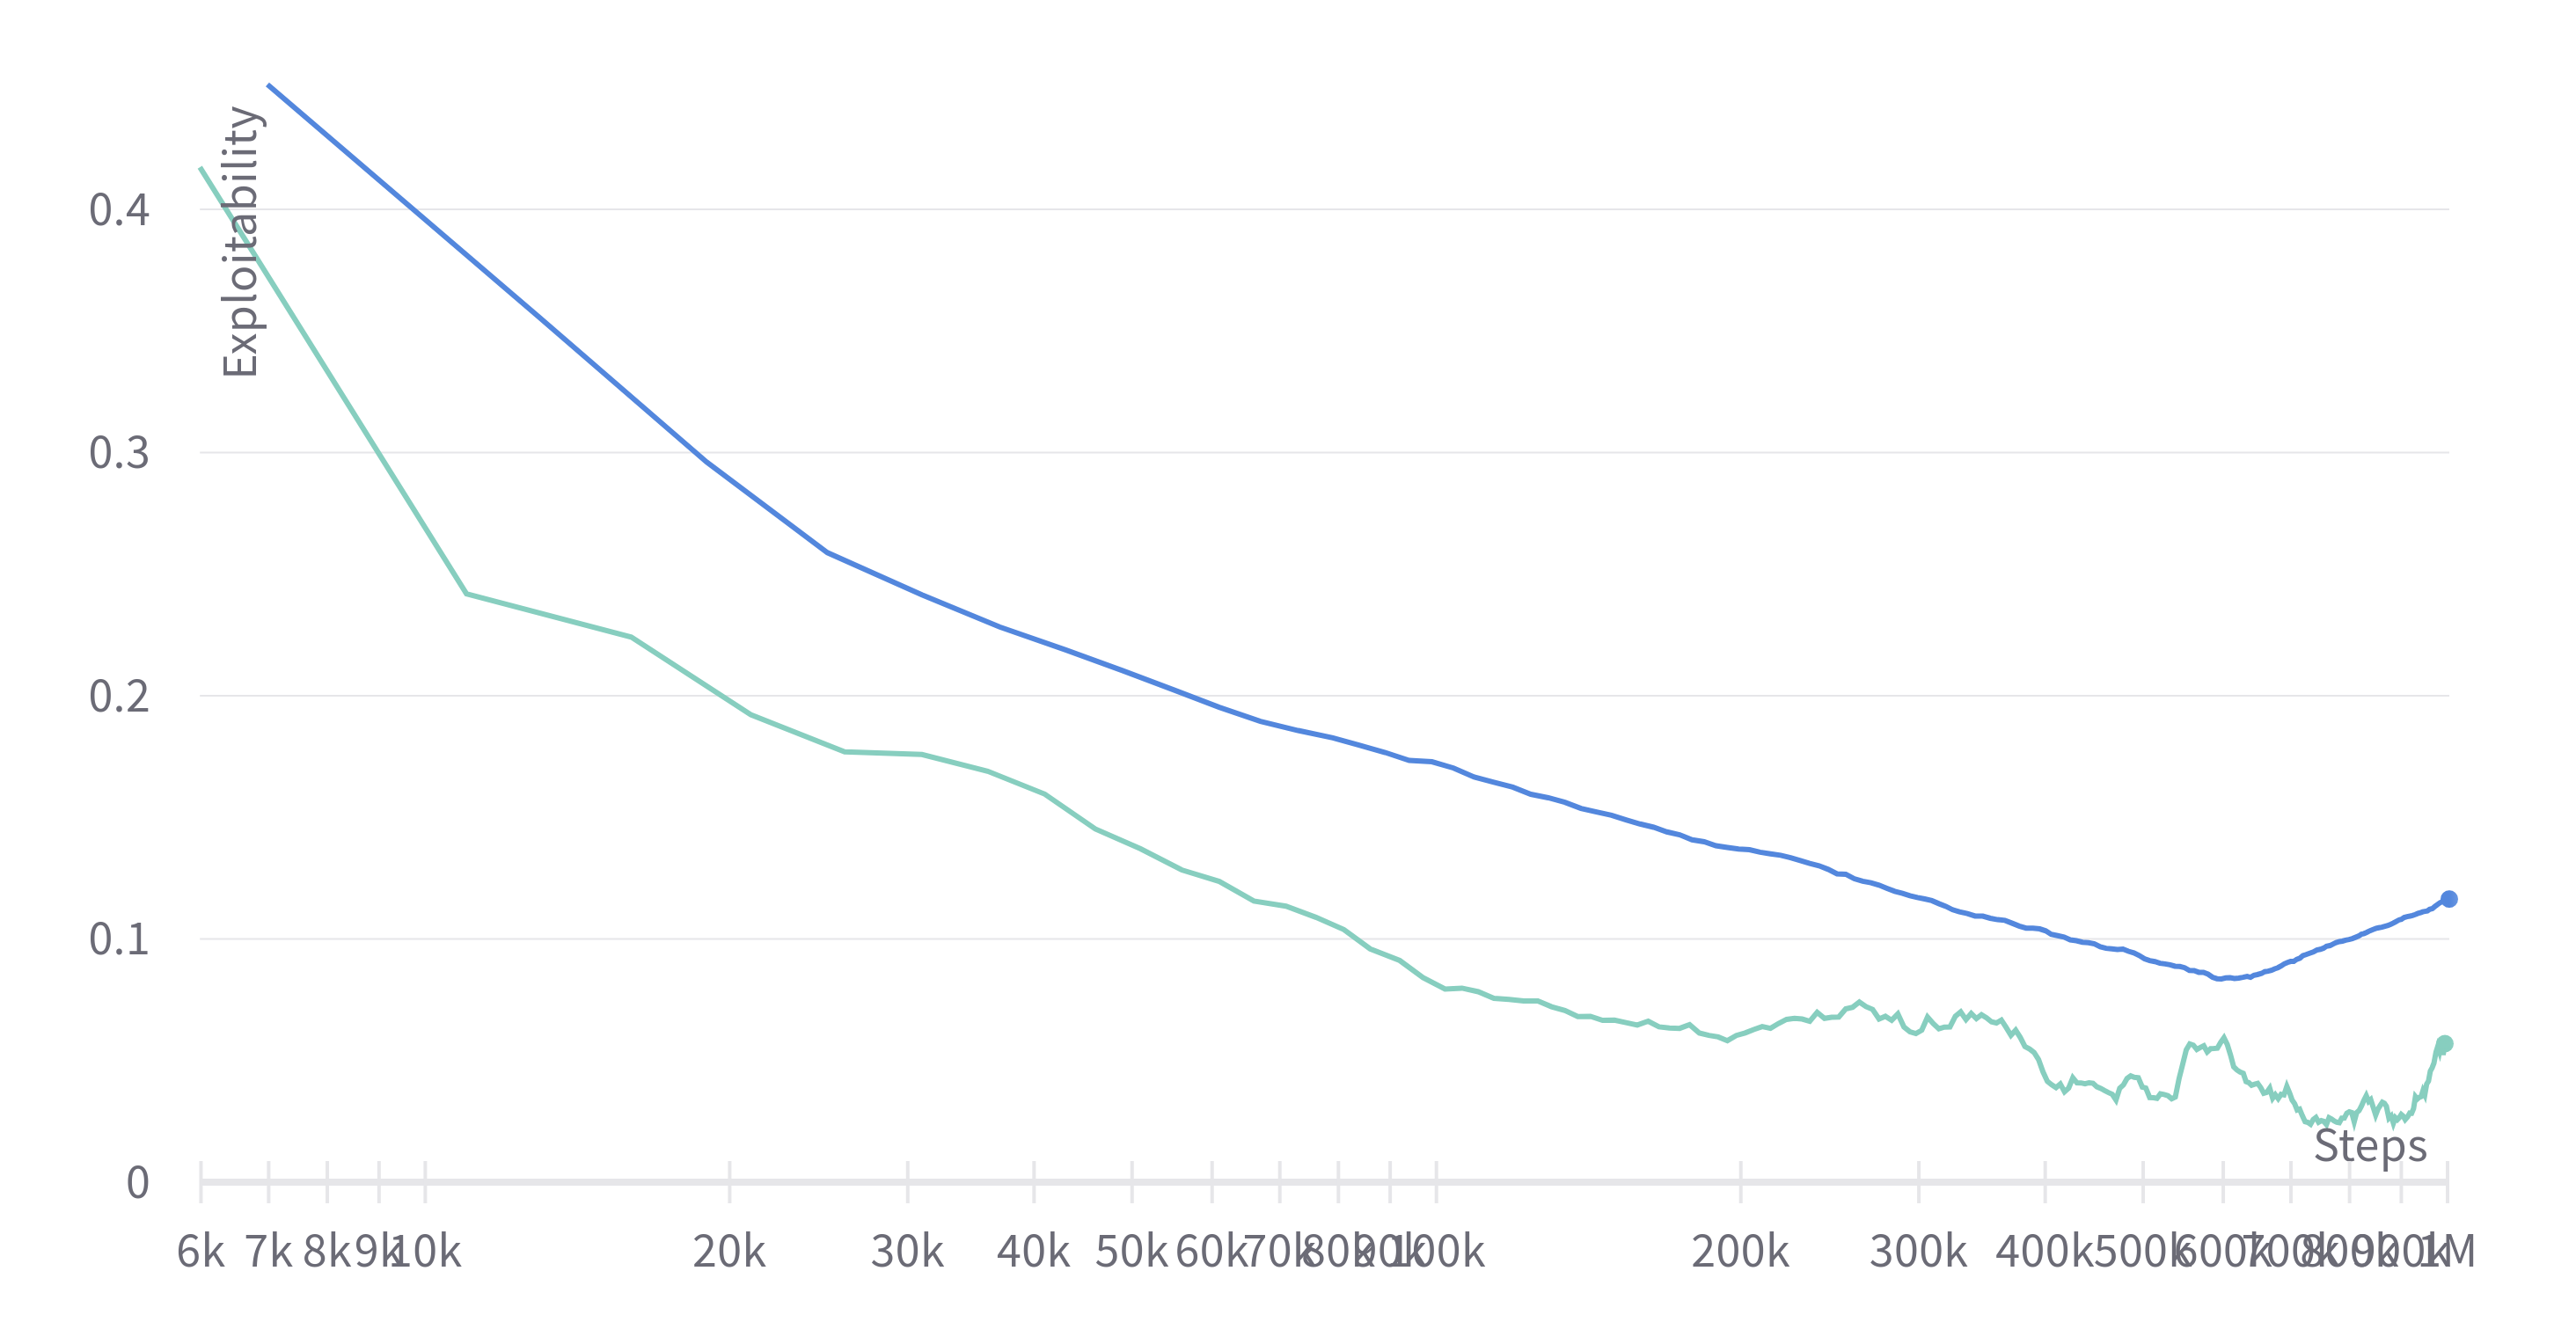
\includegraphics[width=\textwidth]{figs/kpoker.png}
		\caption{Kuhn Poker}
	\end{subfigure}
	\begin{subfigure}[b]{0.6\textwidth}
		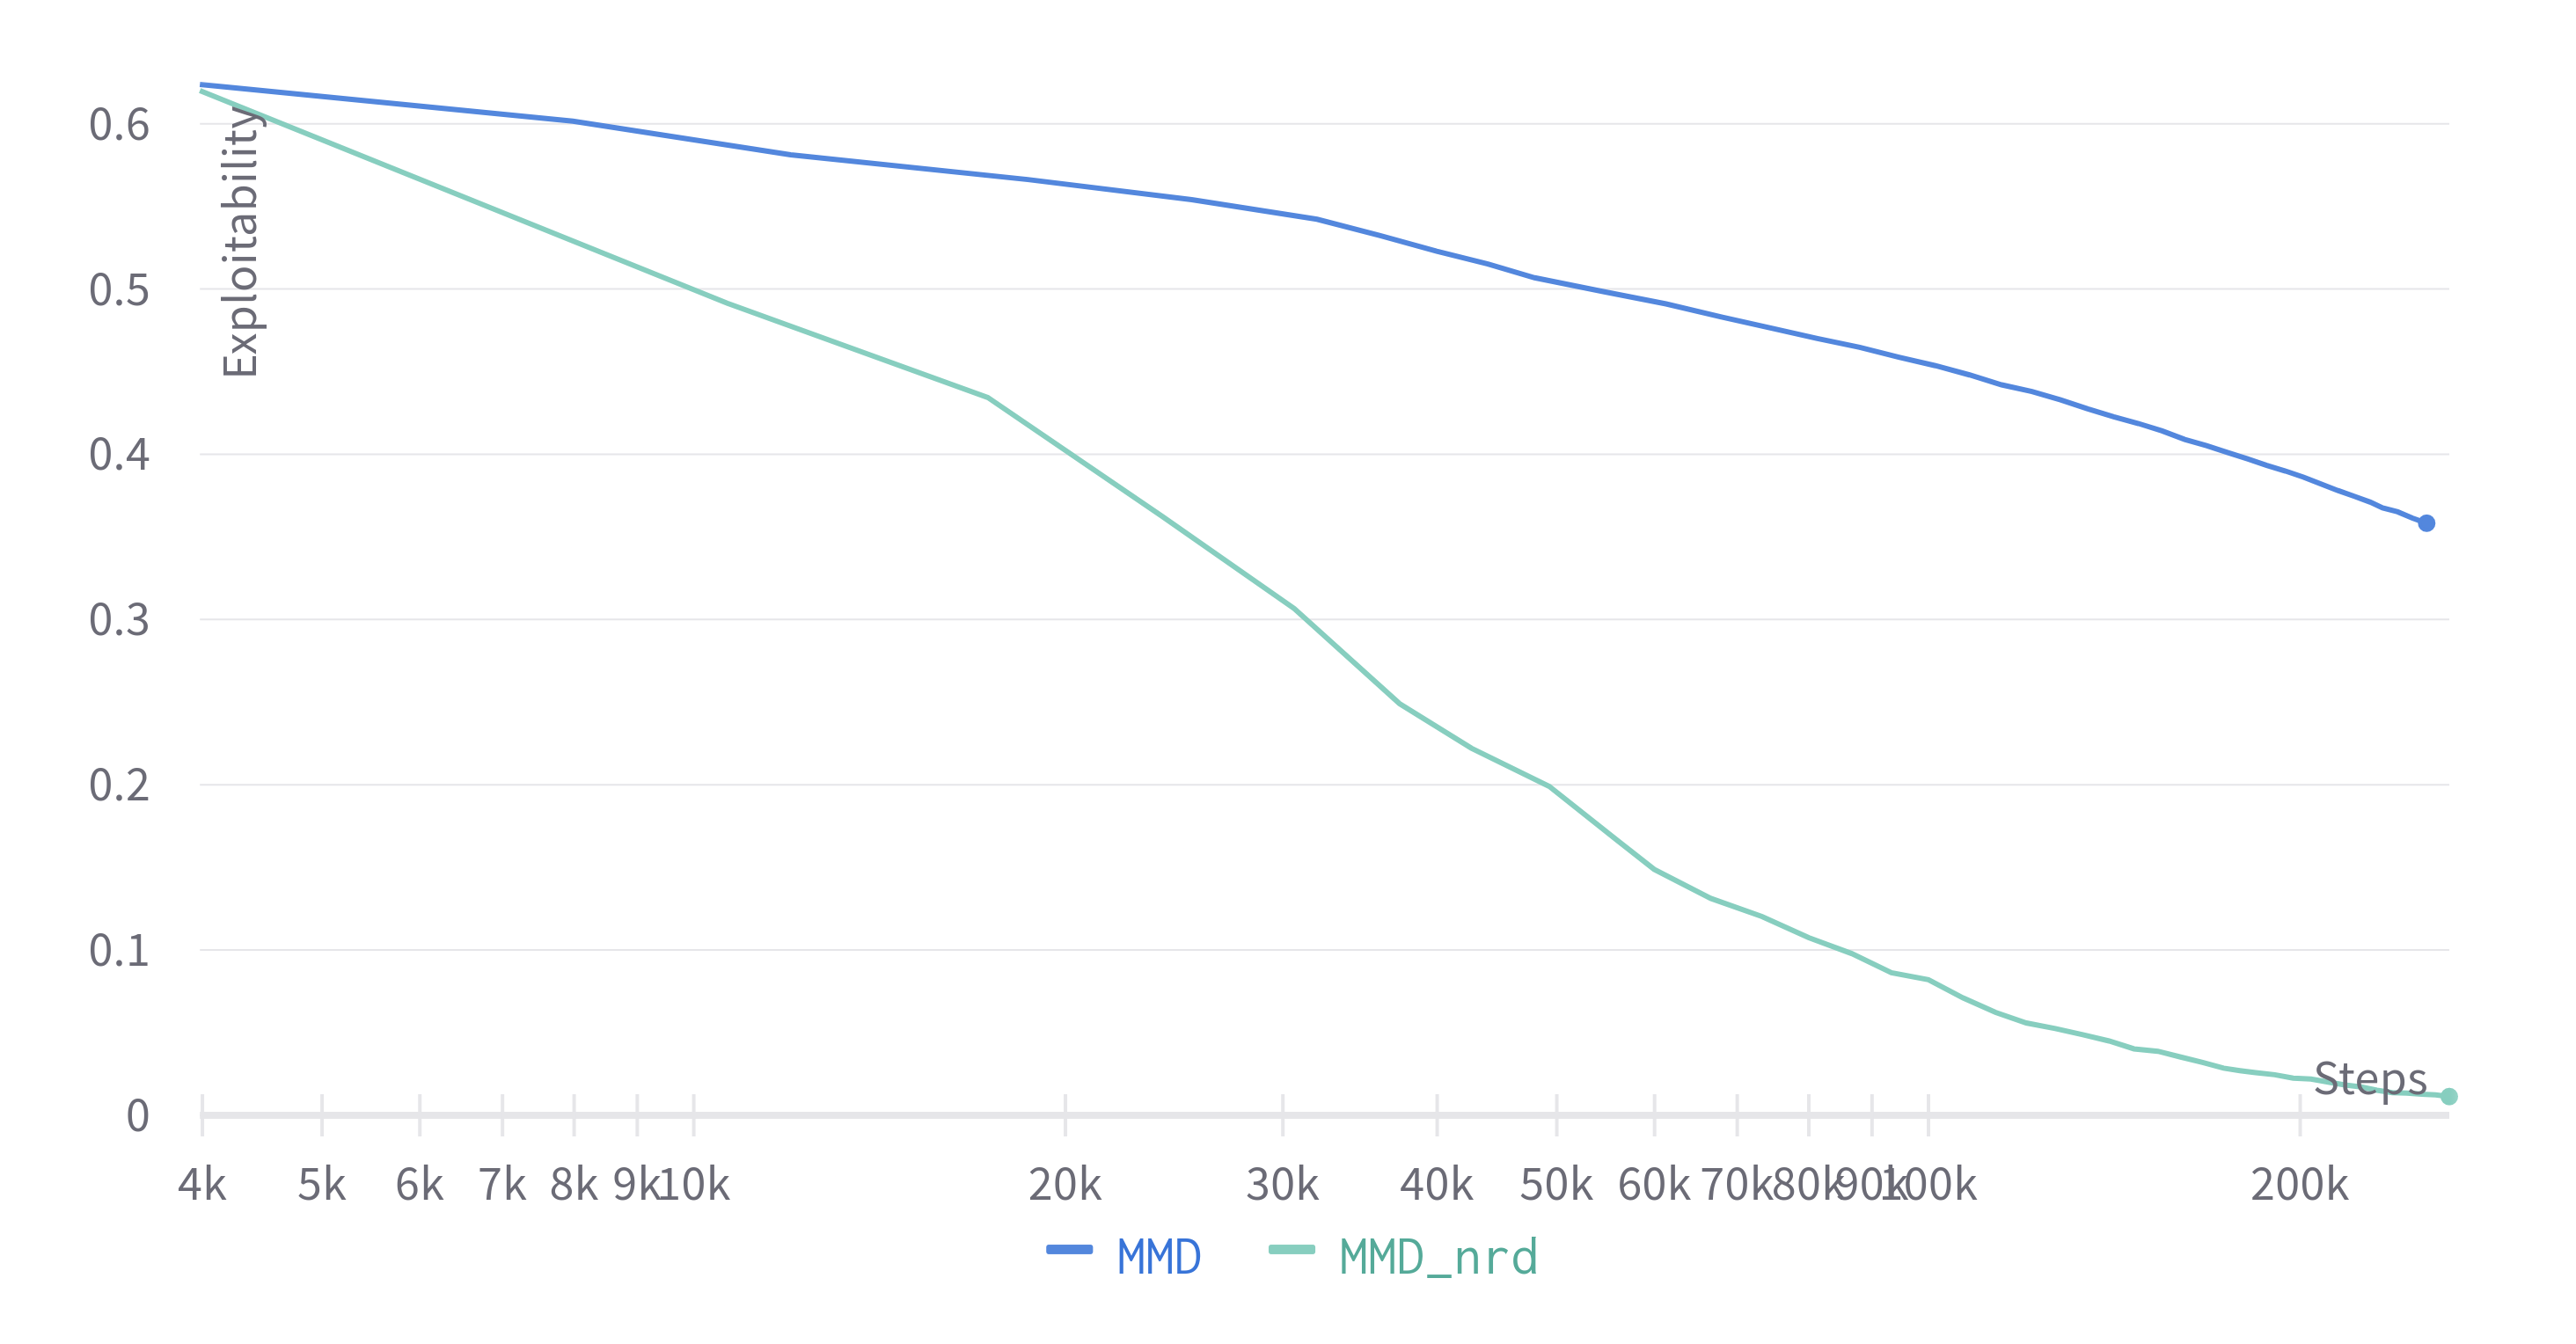
\includegraphics[width=\textwidth]{figs/ahex22.png}
		\caption{Abrupt Dark Hex (2$\times$2) (\red{1M steps version to be added})}
	\end{subfigure}
	\caption{Performance in small EFGs, measured by exact exploitability.}
	\label{fig:neuralsmall1}
\end{figure}

% We also compute approximate exploitability for the smaller games by training a DQN best-response
% agent for 1M steps against the fixed trained agents.

\ref{fig:neural2} shows improvement in performance by applying the NeuRD-fix in Abrupt Dark Hex
(3$\times$3) and Phantom TTT, as measured by the approximate exploitability.
\begin{figure}[H]
	\centering
	\begin{subfigure}[b]{0.4\textwidth}
		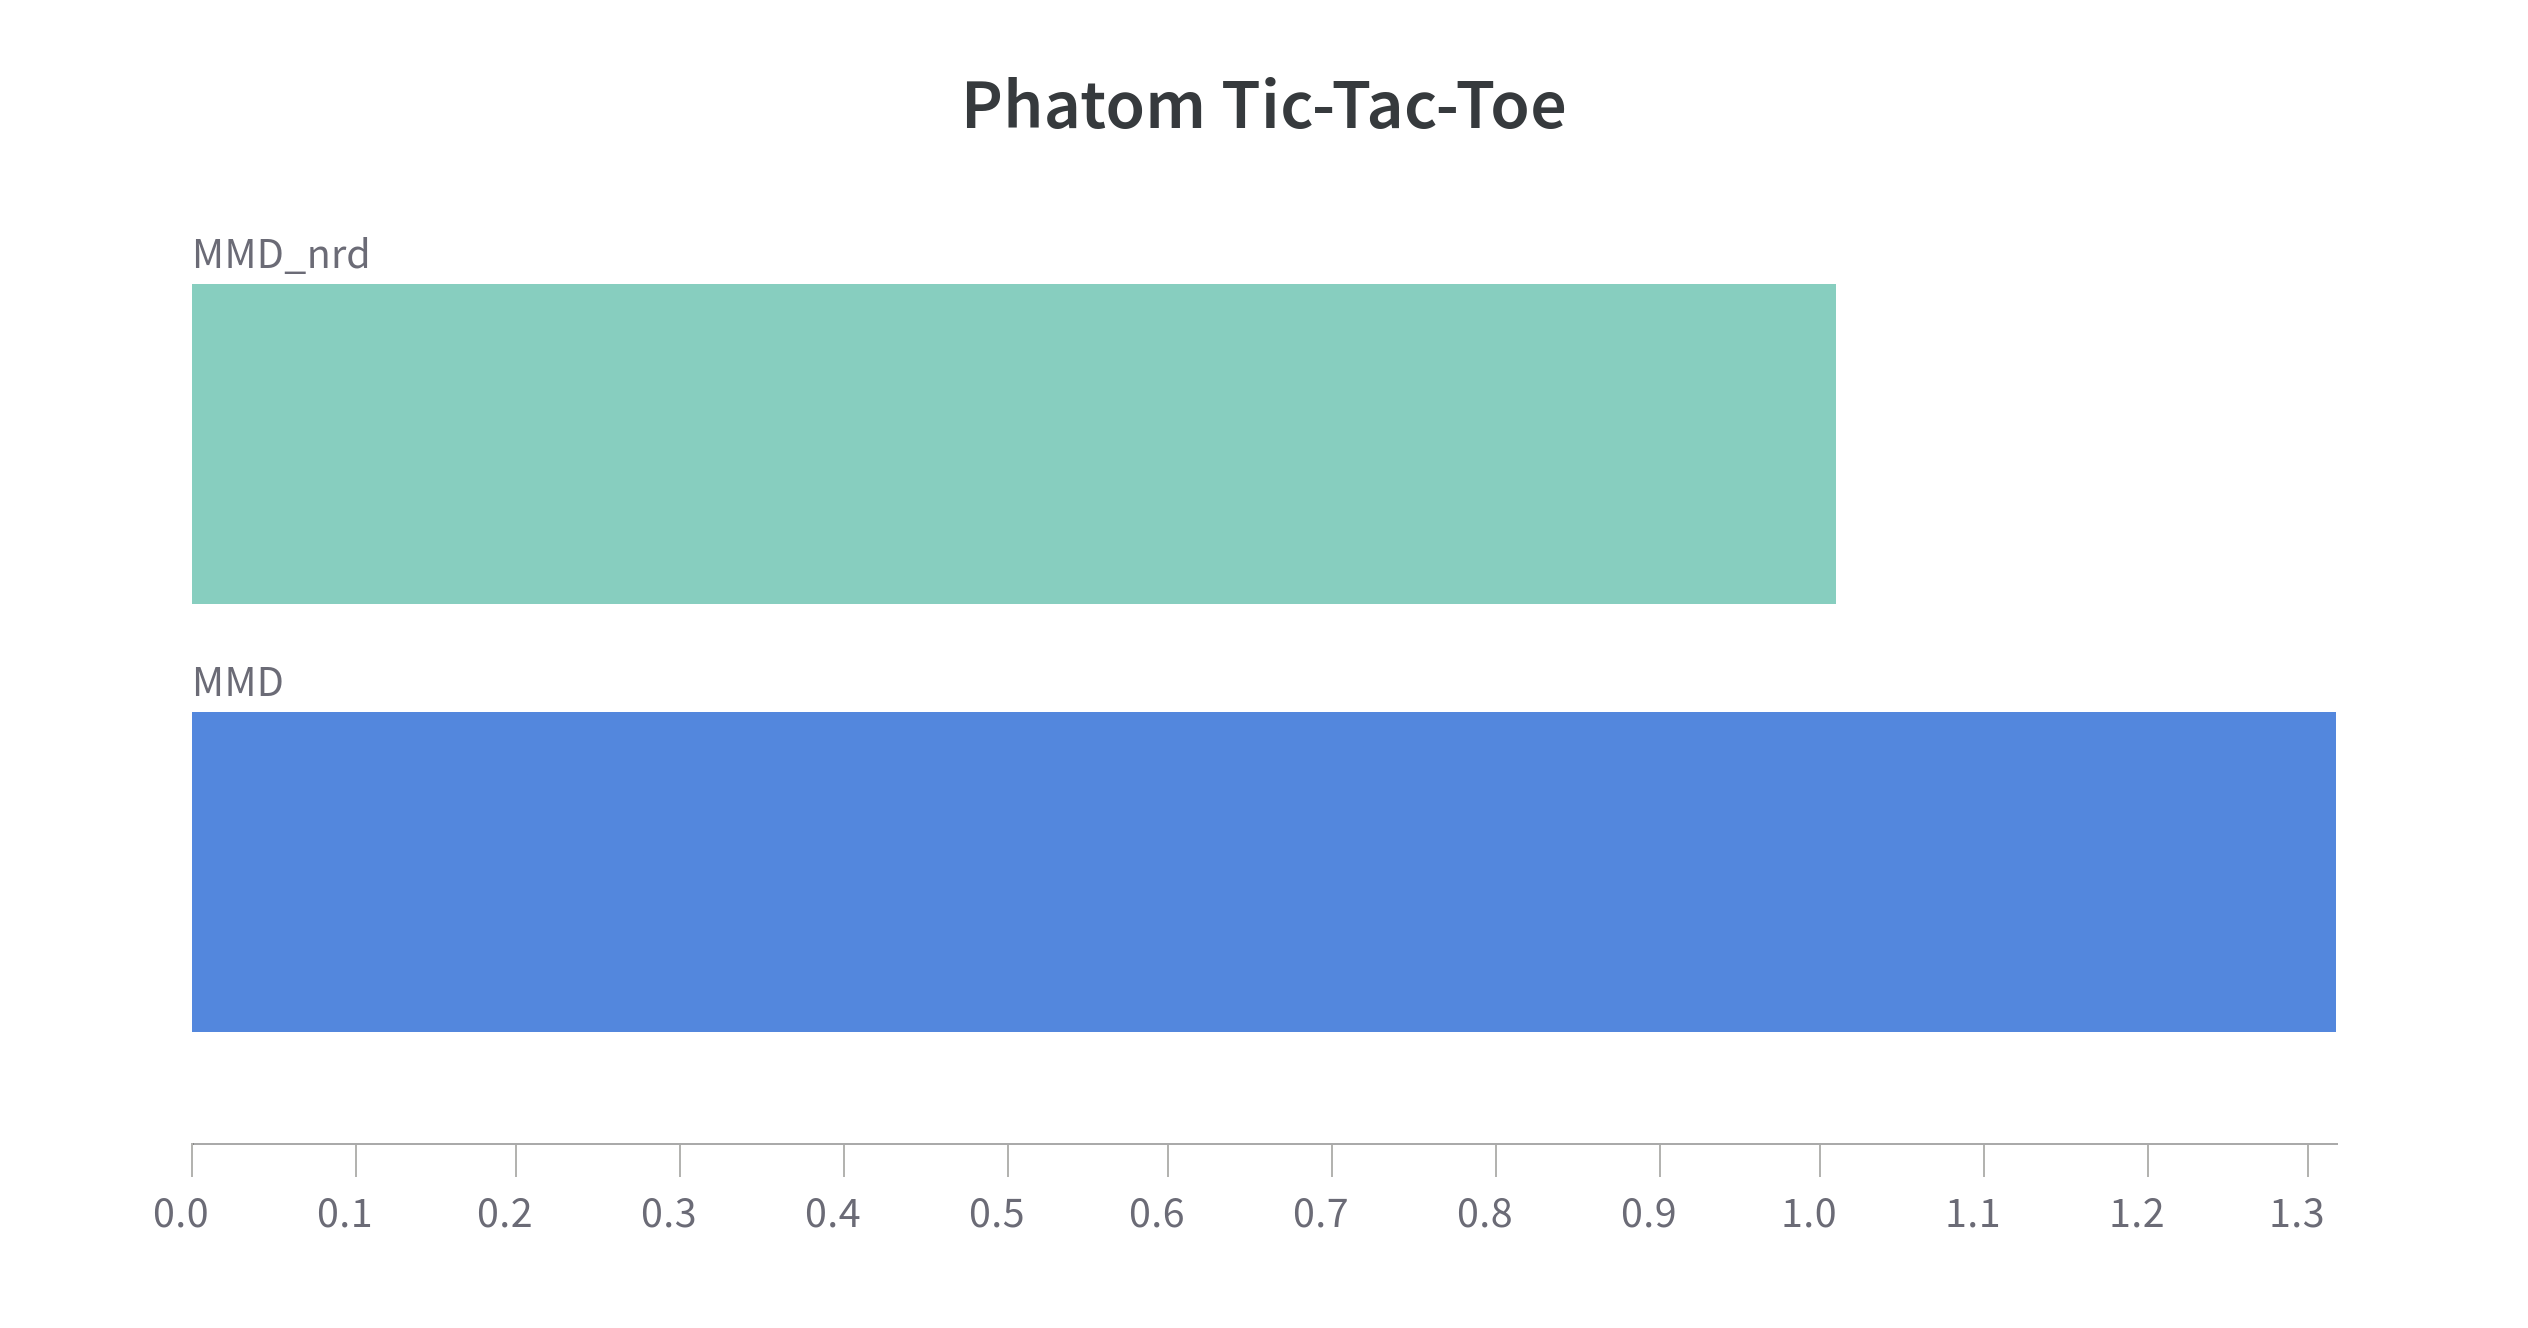
\includegraphics[width=\textwidth]{figs/pttt.png}
		\caption{Phantom Tic-tac-toe}
	\end{subfigure}
	\begin{subfigure}[b]{0.4\textwidth}
		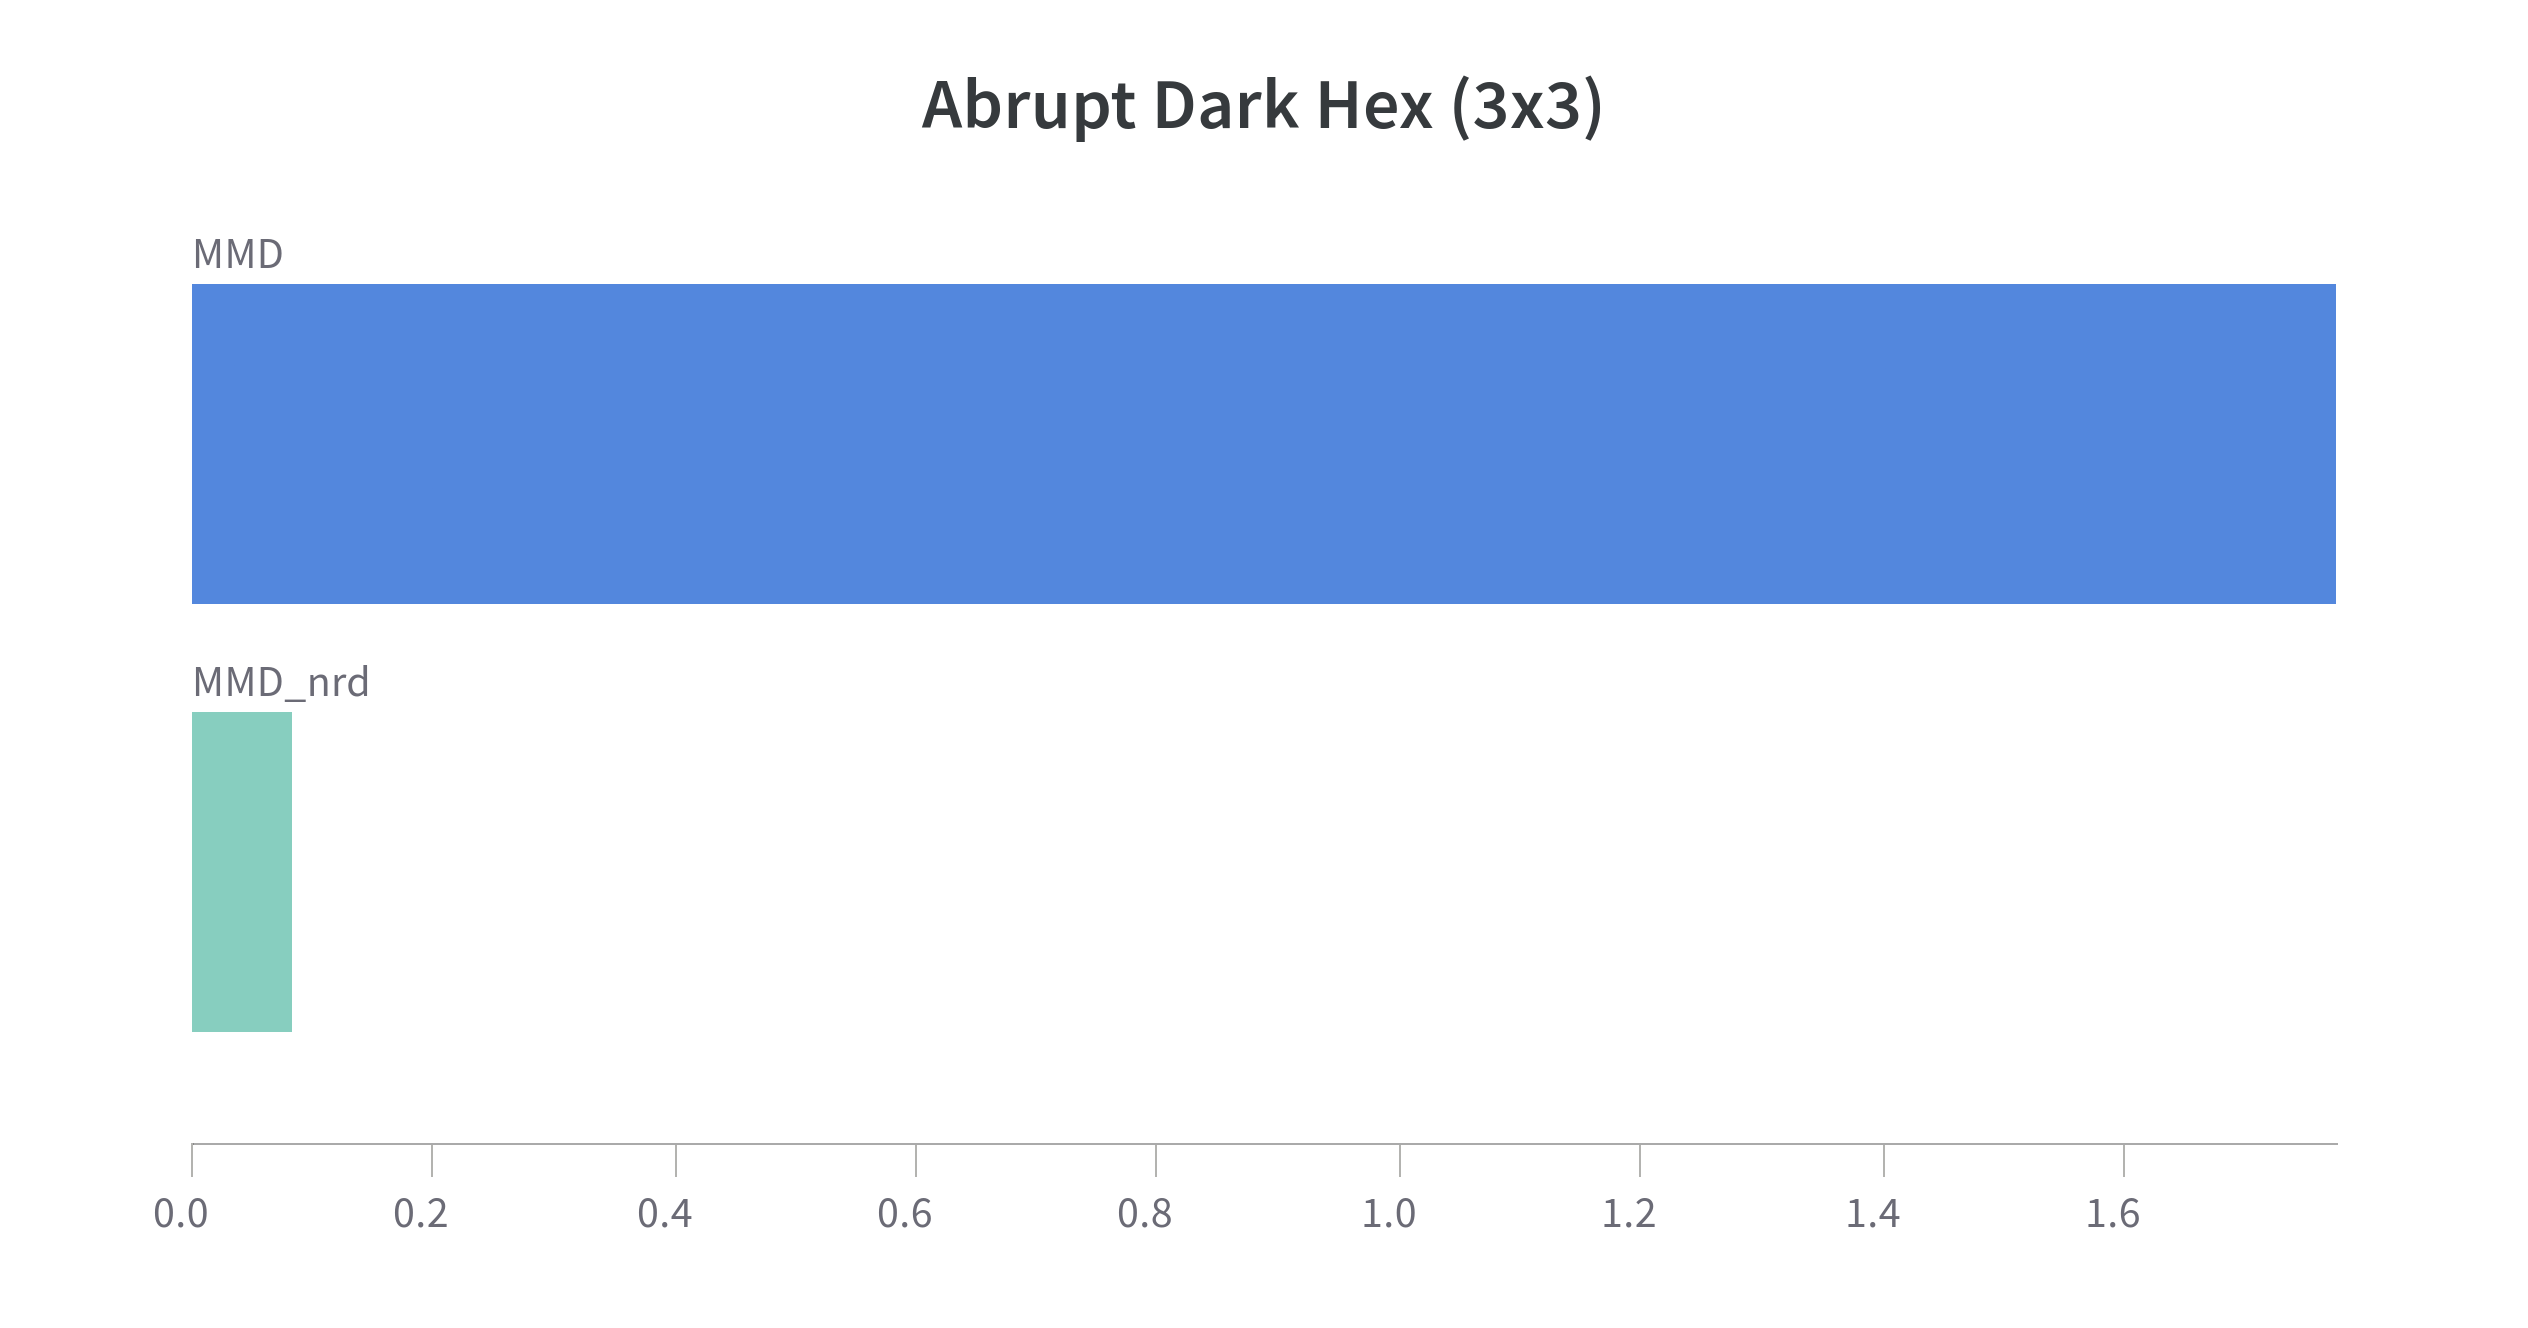
\includegraphics[width=\textwidth]{figs/ahex33.png}
		\caption{Abrupt Dark Hex (3$\times$3)}
	\end{subfigure}
	\caption{Performance in larger EFGs, measured by approximate exploitability.}
	\label{fig:neural2}
\end{figure}

Firstly, echoing the observations from the tabular experiments, we observe that the addition of
NeuRD-fix improved the performance of MMD.
Secondly, there is no consistent benefit of using the optimistic version of the optimizers in
contrast to their effect in normal-form games.

\fillin{We also evaluate these algorithms by having the trained agents play against each other in a
	head-to-head manner.}